%------------------------------------------------------------
\title[14 - 函数Ⅱ]
{14 - 函数Ⅱ}

\subtitle{C++ 程序设计进阶}

\author[Beiyu Li]
{Beiyu Li\\
\texttt{<sysulby@gmail.com>}}

% \institute[SOJ]
% {Sicily Online Judge}

\date[\today]
{\number\year 年 \number\month 月 \number\day 日}
%------------------------------------------------------------


\begin{document}

\author[sysulby]
{SOJ 信息学竞赛教练组}

\begin{frame}
    \titlepage
\end{frame}
\setcounter{framenumber}{0} % 标题页不编号


\section{复习回顾}

%------------------------------------------------------------

% 复习回顾

%------------------------------------------------------------

%------------------------------------------------------------
\begin{frame}[fragile]
    \frametitle{函数的使用场景}

    \alt<2-6>{
        \begin{itemize}
            \item<2-> 多次使用相同功能
            
            \begin{itemize}
                \item<3-> 五边形面积
            \end{itemize}

            \item<4-> 复杂的逻辑嵌套
            
            \begin{itemize}
                \item<5-> 质数判断
            \end{itemize}

        \end{itemize}
    }{
        \begin{block}{}
            \vspace{.5cm}
            \begin{center}
                什么时候使用函数?
            \end{center}
            \vspace{.5cm}
        \end{block}
    }
\end{frame}
%------------------------------------------------------------

%------------------------------------------------------------
\begin{frame}[fragile]
    \frametitle{模块化编程}

    \alt<2-4>{
        \begin{itemize}
            \item<2-> 将一个大程序按照功能划分为若干小程序模块
            \item<3-> 每个小程序模块完成一个确定的功能
            \item<4-> 模块之间建立必要的联系,通过模块的互相协作完成整个程序
        \end{itemize}    
    }{
        \begin{block}{}
            \vspace{.5cm}
            \begin{center}
                如何设计一个函数?
            \end{center}
            \vspace{.5cm}
        \end{block}
    }
\end{frame}
%------------------------------------------------------------

%------------------------------------------------------------
\begin{frame}[fragile]
    \frametitle{例 2.1:五边形面积}

    \alt<6>{
        \lstinputlisting[basicstyle=\ttfamily\scriptsize,language=C++,name=triArea]{ch14/triArea.cc}
    } {
        \alt<5> {
            \begin{exampleblock}{函数解决子任务}
                \begin{itemize}
                    \item 重复的子任务:计算三角形面积
                    \item 函数的定义
                    
                    \begin{itemize}
                        \item 功能:返回边长分别为 $a$, $b$, $c$ 的三角形面积
                        \item 参数:根据题目输入的数据类型和大小确定参数为 \lstinline|int| 类型
                        \item 返回值:三角形面积可能是浮点数,返回值为 \lstinline|double| 类型
                    \end{itemize}

                \end{itemize}

            \end{exampleblock}
        } {
            \alt<3-4>{
                \begin{exampleblock}{细分任务}
                    \begin{itemize}
                        \item 将求解五边形面积这个任务细分为多个子任务,每个子任务为一个模块
                        
                        \begin{columns}[onlytextwidth,T]
                            \column{.05\textwidth}
                            \column{.65\textwidth}
                            \begin{itemize}
                                \item 输入数据
                                \item 计算边长为 $a$, $b$, $c$ 三角形的面积
                                \item 计算边长为 $c$, $d$, $e$ 三角形的面积
                                \item 计算边长为 $e$, $f$, $g$ 三角形的面积
                                \item 计算五边形面积并输出
                            \end{itemize}

                            \begin{tikzpicture}[remember picture, overlay]
                                \uncover<4>{\draw[red, very thick] (0, 1.1) rectangle (5.6, 3.3) node[below, xshift=-.3cm, yshift=-2.8cm]{功能相同的多个子任务,定义一个函数,重复调用即可};}
                            \end{tikzpicture}

                            \column{.30\textwidth}
                            % 图像
                            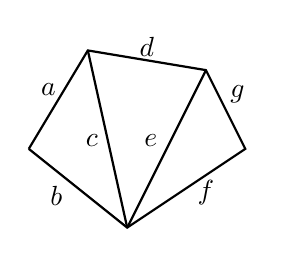
\begin{tikzpicture}
                                \draw[thick] (0.5 / 2,2 / 2) -- (2 / 2,4.5 / 2) -- (5 / 2,4 / 2) -- (6 / 2,2 / 2) -- (3 / 2,0 / 2) -- (0.5 / 2,2 / 2);
                                \draw[thick] (2 / 2,4.5 / 2) -- (3 / 2,0 / 2);
                                \draw[thick] (5 / 2,4 / 2) -- (3 / 2,0 / 2);

                                \node at (1 / 2,3.5 / 2){$a$};
                                \node at (1.2 / 2,0.8 / 2){$b$};
                                \node at (2.1 / 2,2.2 / 2){$c$};
                                \node at (3.5 / 2,4.6 / 2){$d$};
                                \node at (3.6 / 2,2.2 / 2){$e$};
                                \node at (5 / 2,0.9 / 2){$f$};
                                \node at (5.8 / 2,3.4 / 2){$g$};
                            \end{tikzpicture}
                        \end{columns}

                    \end{itemize}

                \end{exampleblock}
            }{
                \alt<2>{
                    \begin{exampleblock}{问题分析}
                        \begin{itemize}
                            \item 一个五边形可以分割为三个三角形,因此五边形的面积等于三个三角形的面积之和
                        \end{itemize}

                        \begin{columns}[onlytextwidth,T]
                            \column{.7\textwidth}
                            \begin{itemize}
                        1        \item 三角形的面积可以套用海伦公式求解
                            \end{itemize}

                            \column{.3\textwidth}
                            % 图像
                            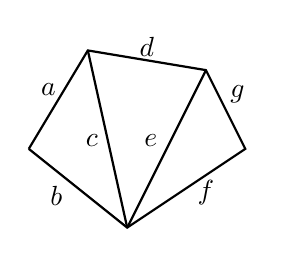
\begin{tikzpicture}
                                \draw[thick] (0.5 / 2,2 / 2) -- (2 / 2,4.5 / 2) -- (5 / 2,4 / 2) -- (6 / 2,2 / 2) -- (3 / 2,0 / 2) -- (0.5 / 2,2 / 2);
                                \draw[thick] (2 / 2,4.5 / 2) -- (3 / 2,0 / 2);
                                \draw[thick] (5 / 2,4 / 2) -- (3 / 2,0 / 2);

                                \node at (1 / 2,3.5 / 2){$a$};
                                \node at (1.2 / 2,0.8 / 2){$b$};
                                \node at (2.1 / 2,2.2 / 2){$c$};
                                \node at (3.5 / 2,4.6 / 2){$d$};
                                \node at (3.6 / 2,2.2 / 2){$e$};
                                \node at (5 / 2,0.9 / 2){$f$};
                                \node at (5.8 / 2,3.4 / 2){$g$};
                            \end{tikzpicture}
                        \end{columns}
                    \end{exampleblock}
                }{

                    \begin{exampleblock}{编程题}
                        \begin{itemize}
                            \item 如图所示的五边形,输入其 $5$ 条边和 $2$ 条对角线的边长,求这个五边形的面积。\\
                                根据海伦公式,边长分别为 $a$, $b$, $c$ 的三角形面积为 $\sqrt{p (p - a) (p - b) (p - c)}$,
                                其中 $p = \frac{a+b+c}{2}$。\\
                                输出结果保留至小数点后两位。
                        \end{itemize}

                        \begin{columns}[onlytextwidth,T]
                            \column{.7\textwidth}
                            \begin{itemize}
                                \item 样例输入
                                
                                    \lstinline|3 4 5 6 7 8 9|

                                \item 样例输出
                                
                                    \lstinline|47.53|
                            \end{itemize}
                            \column{.3\textwidth}
                                % 图像
                                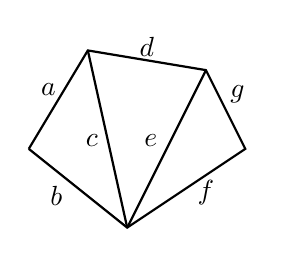
\begin{tikzpicture}
                                    \draw[thick] (0.5 / 2,2 / 2) -- (2 / 2,4.5 / 2) -- (5 / 2,4 / 2) -- (6 / 2,2 / 2) -- (3 / 2,0 / 2) -- (0.5 / 2,2 / 2);
                                    \draw[thick] (2 / 2,4.5 / 2) -- (3 / 2,0 / 2);
                                    \draw[thick] (5 / 2,4 / 2) -- (3 / 2,0 / 2);

                                    \node at (1 / 2,3.5 / 2){$a$};
                                    \node at (1.2 / 2,0.8 / 2){$b$};
                                    \node at (2.1 / 2,2.2 / 2){$c$};
                                    \node at (3.5 / 2,4.6 / 2){$d$};
                                    \node at (3.6 / 2,2.2 / 2){$e$};
                                    \node at (5 / 2,0.9 / 2){$f$};
                                    \node at (5.8 / 2,3.4 / 2){$g$};
                                \end{tikzpicture}
                        \end{columns}
                    \end{exampleblock}

                }
            }
        }
    }

\end{frame}
%------------------------------------------------------------

%------------------------------------------------------------
\begin{frame}[fragile]
    \frametitle{例 2.2:质数判断}

    \alt<6-8> {
        \begin{columns}[onlytextwidth,T]
            \column{.7\textwidth}
            \lstinputlisting[basicstyle=\ttfamily\scriptsize,language=C++,name=isPrime_2]{ch14/isPrime_2.cc}

            \begin{tikzpicture}[remember picture, overlay]
                \uncover<8>{\redbox{isPrime_2}{9}{14}{9}{14} node[right,xshift=.5cm,yshift=-0.7cm]{如果 $n$ 是 \lstinline|long long| 类型,怎么修改?};}
            \end{tikzpicture}

            \column{.3\textwidth}
            \begin{itemize}
                \item<7-> 时间复杂度 $O(\sqrt{n})$
            \end{itemize}
        \end{columns}

    } {
    \alt<5>{
        \begin{exampleblock}{质数判定的优化}
            \begin{itemize}
                \item 观察一个数字除了 $1$ 和它本身之外的因数,例如 $36$
                
                \begin{itemize}
                    \item $2, 3, 4, 6, 9, 12, 18$
                    \item 因数是成对存在的:$2 \times 18 = 36$, $3 \times 12 = 36$, ...
                \end{itemize}

                \item 成对的两个因数,其中一个 $\leq \sqrt{n}$ ,一个 $\geq \sqrt{n}$ 
                \item 如果 $n$ 不存在 $\leq \sqrt{n}$ 的因数,肯定也不存在 $\geq \sqrt{n}$ 的因数
                \item 所以判定质数代码中的 $i$ 只需要枚举到 $\sqrt{n}$ ,不用枚举到 $n - 1$
            \end{itemize}
        \end{exampleblock}
    } {
        \alt<3-4>{
            \begin{itemize}
                \item 判断 $n$ 有没有 $2 \sim n - 1$ 范围的因数
            \end{itemize}

            \lstinputlisting[basicstyle=\ttfamily\scriptsize,language=C++,name=isPrime_1]{ch14/isPrime_1.cc}

            \begin{tikzpicture}[remember picture, overlay]
                \uncover<4>{\redbox{isPrime_1}{2}{5}{2}{30} node[right,xshift=.5cm,yshift=.2cm]{是否正确?};}
            \end{tikzpicture}
        } {
            \alt<2>{
                \begin{exampleblock}{质数基本概念}
                    \begin{itemize}
                        \item 整除:指整数 $a$ 除以整数 $b$ ($b \neq 0$) 的余数为 $0$ 
                        \item 因数(约数):如果 $a$ 除以 $b$ 能够整除,则 $b$ 是 $a$ 的因数(约数)
                        \item 倍数:如果 $a$ 除以 $b$ 能够整除,则 $a$ 是 $b$ 的倍数
                        \item 质数(素数):指在大于 $1$ 的自然数中,除了 $1$ 和它本身以外不再有其他因数的自然数
                    \end{itemize}
                \end{exampleblock}
            } {
                \begin{exampleblock}{编程题}
                    \begin{itemize}
                        \item 输入一个正整数 $n$ ($1 \leq n \leq 2 \times 10^9$),判断 $n$ 是否为质数。\\
                            若 $x$ 是质数,输出 \lstinline|yes|;否则输出 \lstinline|no|。
                        \item 样例输入
                                            
                            \lstinline|3|

                        \item 样例输出
                        
                            \lstinline|yes|
                
                    \end{itemize}
                \end{exampleblock}
            }
        }
    }
    }
\end{frame}
%------------------------------------------------------------

%------------------------------------------------------------
\begin{frame}[fragile]
    \frametitle{使用函数的优点}

        \begin{itemize}
            \item 将功能封装到函数中,提高代码的可读性
            \item 提高代码的复用性,使代码简洁
            \item 将代码分解成更小的块(模块化),使代码逻辑简单明了,易于查错
        \end{itemize}
    
\end{frame}
%------------------------------------------------------------

% 变量的作用域
%------------------------------------------------------------
\begin{frame}[fragile]
    \frametitle{变量的作用域}

        \begin{itemize}
            \item<1-> 代码中的变量并不是在任何位置都可以使用
            \item<2-> 一个变量可用的代码范围就是这个变量的作用域
            \item<3-> 根据作用域的不同,可以把变量分为局部变量和全局变量
        \end{itemize}
    
\end{frame}
%------------------------------------------------------------

% 局部变量的定义
%------------------------------------------------------------
\begin{frame}[fragile]
    \frametitle{局部变量}

        \begin{itemize}
            \item 声明在函数内部的变量
            \item 作用域:从变量的声明开始到包含它的块结束

            \begin{itemize}
                \item 块是用一对花括号括起来的代码区域
                \item 循环、分支语句(包含条件语句)视作一个块
                \item 函数(包含参数列表)也视作一个块
            \end{itemize}
            
        \end{itemize}
    
\end{frame}
%------------------------------------------------------------

% 局部变量的动画讲解
%------------------------------------------------------------

%------------------------------------------------------------

% 全局变量的定义
%------------------------------------------------------------
\begin{frame}[fragile]
    \frametitle{全局变量}

        \begin{itemize}
            \item 定义在所有函数外部、没有被任何花括号包含起来的变量
            \item 作用域:从变量的声明开始一直到代码结束,作用域中任意的函数都可以使用该变量
        \end{itemize}
    
\end{frame}
%------------------------------------------------------------

% 全局变量的动画讲解
%------------------------------------------------------------

%------------------------------------------------------------

% 同名变量的定义
%------------------------------------------------------------
\begin{frame}[fragile]
    \frametitle{同名变量}

        \begin{itemize}
            \item 在同一个“块”里面声明的同名变量冲突
            \item 在不同“块” 里面声明的同名变量不冲突

            \begin{itemize}
                \item 完全覆盖
                \item 完全不覆盖
            \end{itemize}
            
        \end{itemize}
    
\end{frame}
%------------------------------------------------------------

% 同名变量的动画讲解
%------------------------------------------------------------

%------------------------------------------------------------

% 引用变量
%------------------------------------------------------------
\begin{frame}[fragile]
    \frametitle{引用变量}

    \alt<2-3>{
        \begin{itemize}
            \item<2-> 一般变量

            \begin{itemize}
                \item 一般变量在声明时,会被分配一个独立的内存空间
            \end{itemize}
            
            \item<3-> 引用变量

            \begin{itemize}
                \item 引用变量是其他变量的别名,与其他变量共用同一块内存空间
                \item 在变量类型和变量名之间加一个 & ,表示该变量是一个引用
                \begin{itemize}
                    \item 变量类型 &引用变量名 = 被引用的变量名;
                    \item 引用需要在声明的时候进行初始化,与一个固定的变量绑定
                \end{itemize}
            \end{itemize}
            
        \end{itemize}    
    }{
        \begin{block}{}
            \vspace{.5cm}
            \begin{center}
                两个变量可以用相同名称,\\
                那么同一个变量可不可以有不同名称?
            \end{center}
            \vspace{.5cm}
        \end{block}
    }
\end{frame}
%------------------------------------------------------------

% 引用变量的动画讲解
%------------------------------------------------------------

%------------------------------------------------------------

% 引用变量的应用
%------------------------------------------------------------
\begin{frame}[fragile]
    \frametitle{引用变量}

    \alt<2-4>{
        % 代码动画
    }{
        \begin{block}{}
            \vspace{.5cm}
            \begin{center}   
                交换两个变量的值,如何用函数实现?
            \end{center}
            \vspace{.5cm}
        \end{block}
    }
\end{frame}
%------------------------------------------------------------

% 参数传递的定义
%------------------------------------------------------------
\begin{frame}[fragile]
    \frametitle{参数传递}

        \begin{itemize}
            \item 按值传递

            \begin{itemize}
                \item 若参数声明为一般形式,参数传递时只是将实参的数值赋值给形参,函数不能访问实参本身
            \end{itemize}
            
            \item 按引用传递

            \begin{itemize}
                \item 引用变量是其他变量的别名,与其他变量共用同一块内存空间
                \item 将形式参数声明为引用类型,可以访问和修改实参本身
            \end{itemize}
            
        \end{itemize}
    
\end{frame}
%------------------------------------------------------------

% 交换变量的值动画讲解
%------------------------------------------------------------

%------------------------------------------------------------

% 参数传递的总结
%------------------------------------------------------------
\begin{frame}[fragile]
    \frametitle{参数传递}

        \begin{itemize}
            \item 按值传递

            \begin{itemize}
                \item 传递的是数值,形参与实参是不同变量,修改形参不影响实参
                \item 不需要在函数中修改实参时使用
            \end{itemize}
            
            \item 按引用传递

            \begin{itemize}
                \item 传递变量本身,形参与实参是同一个变量
                \item 需要在函数中修改实参时使用
            \end{itemize}
            
        \end{itemize}
    
\end{frame}
%------------------------------------------------------------

% 数组传递
%------------------------------------------------------------
\begin{frame}[fragile]
    \frametitle{数组参数传递}

    

    \alt<2-4>{
        \begin{itemize}
            \item<2-> 按值传递 ?

            \begin{itemize}
                \item 把实参数组所有元素复制到形参数组中,需要付出的时间和储存空间代价过大
                \item C++ 不支持按值传递数组
            \end{itemize}
            
            \item 函数传递数组默认用类似按引用传递的方式

            \begin{itemize}
                \item 形参格式:数据类型 数组名[ ]
                \item 不需要使用引用传递
            \end{itemize}
            
        \end{itemize}
    }{
        \begin{block}{}
            \vspace{.5cm}
            \begin{center}   
                参数是数组,应该按什么方式传递?
            \end{center}
            \vspace{.5cm}
        \end{block}
    }
\end{frame}
%------------------------------------------------------------

\end{document}
